
\documentclass[11 pt,t]{beamer}
\usepackage{verbatim}
\usepackage{latexsym}
\usepackage{amsfonts,amssymb}
\graphicspath{{figures/}}    
\usetheme[
	bullet=circle,		% Other option: square
	bigpagenumber,		% circled page number on lower right
	topline=true,		% colored bar at the top of the frame 
	]{Zurich}


%-----------------------------------------------------------------------------
% DOCUMENT PROPERTIES
\logo{
\includegraphics[scale=0.13]{ouclogo.png}}
\author{DingHao}
\title{Structure of DIP and Fourier Transformation}

%-----------------------------------------------------------------------------


\begin{document}


% ----------------------------------------------------------------------------
\frame{\titlepage}
\frame{\frametitle{Contents}\tableofcontents}
% ----------------------------------------------------------------------------


\section{DIP}

% ----------------------------------------------------------------------------

\begin{frame}
\frametitle{DIP}
\framesubtitle{Structure}
   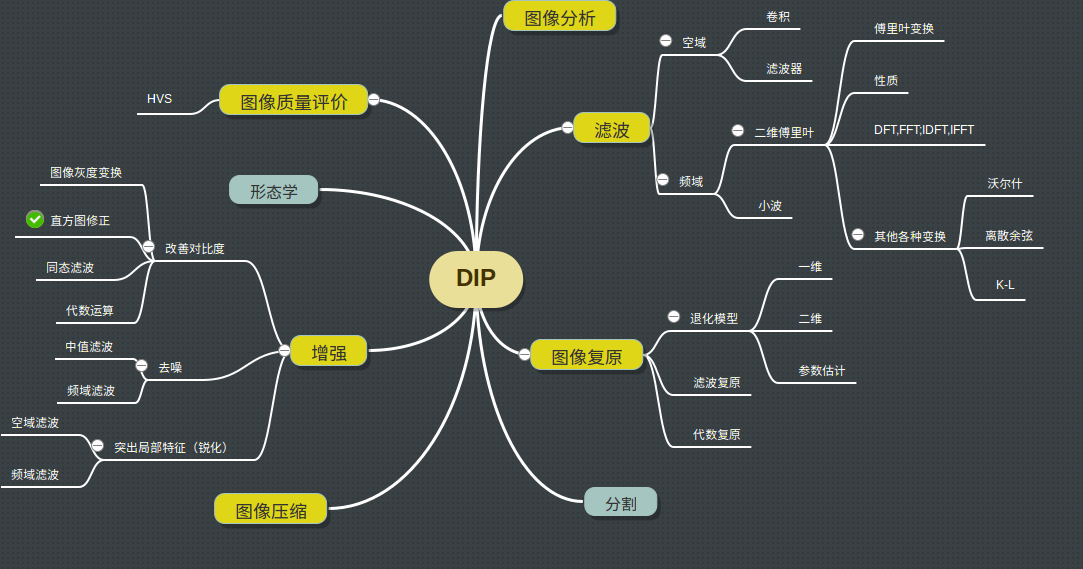
\includegraphics[width=11.3cm]{DIP.png}
\end{frame}

\begin{frame}
\frametitle{DIP}
\framesubtitle{Image quality evaluation}
\begin{itemize}
    \item Subjective
    \item Objective\\
    \item HVS\\
        {\textcolor{tangocolordarkchameleon}{Sensitiveness\\Brightness\\CSF\\Mach effect\\Masking effect} }
\end{itemize}	
\end{frame}

\begin{frame}
\frametitle{DIP}
\framesubtitle{Mathhematical manipulation}
	\begin{itemize}
	\item Fourier
    	\item Gabor\\
{\textcolor{tangocolordarkchameleon}{Compress\\Reinforce\\Merge\\Detection} }
\end{itemize}
\end{frame}

\begin{frame}
\frametitle{DIP}
\framesubtitle{Reinforce}
\begin{itemize}
    \item Improve contrast\\
 {\textcolor{tangocolordarkchameleon}{Grey-scale transformation\\} }
 {\textcolor{tangocolordarkscarletred}{Histogram modification}}
    \item Denoising\\
 {\textcolor{tangocolordarkchameleon}{Masking\\Median filter} }\\
 {\textcolor{tangocolordarkscarletred}{Gabor\\BM3D}}
    \item Sharpen\\
 {\textcolor{tangocolordarkchameleon}{Differential\\Masking} }
\end{itemize}
\end{frame}

\begin{frame}
\frametitle{DIP}
\framesubtitle{Recovery}
Degradation mechanism\\
Filter restoration\\
Algobraic restoration
\end{frame}

% ----------------------------------------------------------------------------

\section{Fourier Transformation}
% ----------------------------------------------------------------------------
\begin{frame}
\frametitle{Fourier Transformation}
\subtitle{structure}
\begin{block}{Formula}
    FT , DFT , 2-D FT , 2-D DFT
\end{block}
\begin{exampleblock}{Character}
    Shift , periodicity , ...
\end{exampleblock}
\begin{alertblock}{Calculation}
    DFT \& IDFT
\end{alertblock}
\end{frame}
% ----------------------------------------------------------------------------

\begin{frame}
\frametitle{Fourier Transformation}
\framesubtitle{Formular}
    $$	F(u,v)=\sum\limits_{x=0}^{M-1}\sum\limits_{y=0}^{N-1}f(x,y)e^{-j2\pi(\frac{ux}{M}+\frac{vy}{N})}$$
   $$u=0,1,2,...,M-1$$$$v=0,1,2,...,N-1$$
\end{frame}

\begin{frame}
\frametitle{Fourier Transformation}
\framesubtitle{2-D DFT}
\begin{figure}
   
\includegraphics[width=6cm]{src.jpg}
\caption{src}
 \end{figure}
\end{frame}

\begin{frame}
\frametitle{Fourier Transformation}
\framesubtitle{2-D DFT}
Move to centre:\\
   $$f(x,y)(-1)^{x+y}\Longleftrightarrow F(u-\frac{M}{2},\frac{N}{2})$$

\end{frame}

\begin{frame}
\frametitle{Fourier Transformation}
\framesubtitle{2-D DFT}
\begin{minipage}[t]{0.4\linewidth}
\begin{figure}
   
\includegraphics[width=5cm]{fourier}
\caption{fourier}
 \end{figure}
        \end{minipage}
\begin{minipage}[t]{0.4\linewidth}
\begin{figure}
   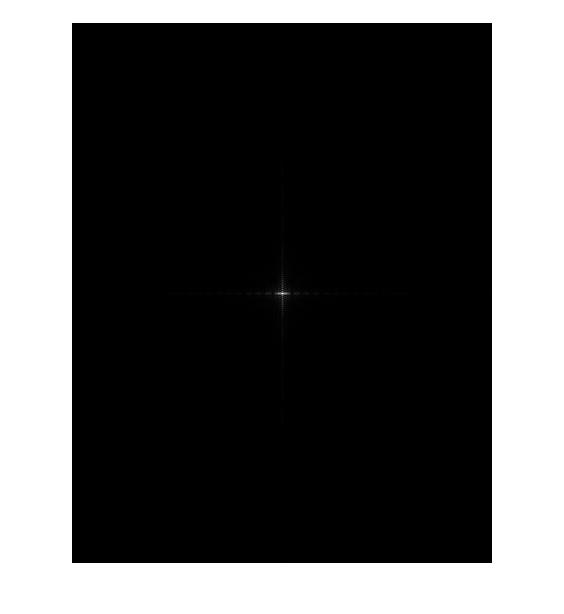
\includegraphics[width=5cm]{centre}
\caption{centre}
 \end{figure}
        \end{minipage}
\end{frame}

\begin{frame}
\frametitle{Fourier Transformation}
\framesubtitle{2-D DFT}
Amplitude:\\
$$\mid F(u,v)\mid =[R(u,v)^{2}+I(u,v)^{2}]^\frac{1}{2}$$
Phase:\\
$$\varphi (u,v)=tan^{-1}[\frac{I(u,v)}{R(u,v)}]$$
\end{frame}

\begin{frame}
\frametitle{Fourier Transformation}
\framesubtitle{2-D DFT}
\begin{minipage}[t]{0.4\linewidth}
\begin{figure}
   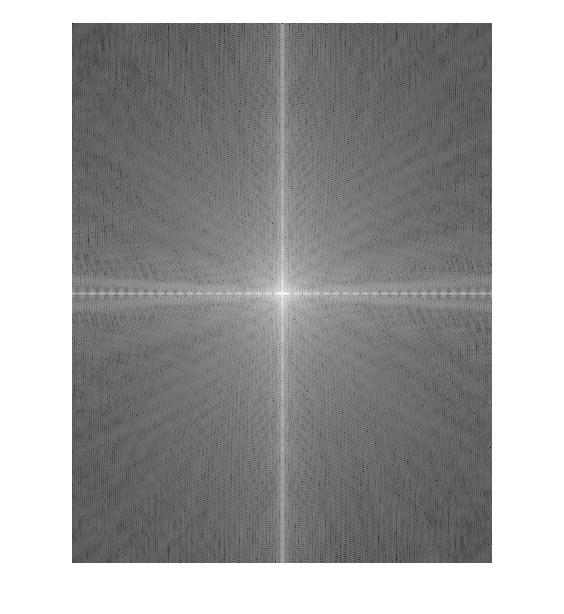
\includegraphics[width=5cm]{amplitude}
\caption{amplitude}
 \end{figure}
        \end{minipage}
\begin{minipage}[t]{0.4\linewidth}
\begin{figure}
   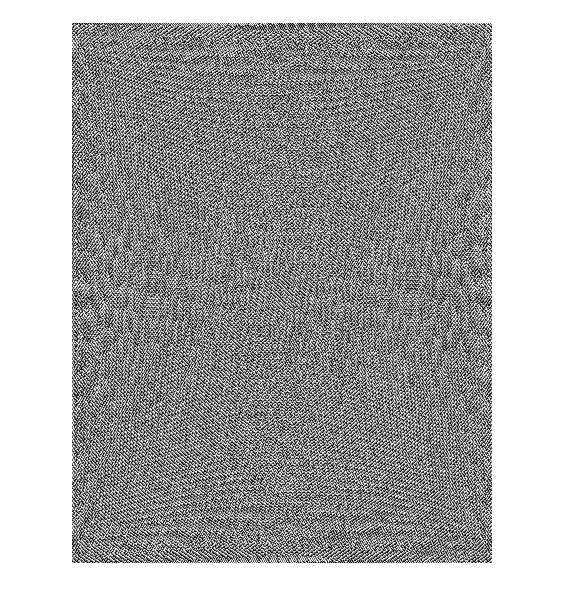
\includegraphics[width=5cm]{phase}
\caption{phase}
 \end{figure}
        \end{minipage}
\end{frame}

\begin{frame}
\frametitle{Fourier Transformation}
\framesubtitle{2-D DFT}
\begin{minipage}[t]{0.4\linewidth}
\begin{figure}
   
\includegraphics[width=5cm,height=5.8cm]{back}
\caption{inverse fourier}
 \end{figure}
        \end{minipage}
\begin{minipage}[t]{0.4\linewidth}
\begin{figure}
   
\includegraphics[width=5cm,height=5.8cm]{sub}
\caption{subtraction}
 \end{figure}
        \end{minipage}
\end{frame}

\begin{frame}
\frametitle{Fourier Transformation}
\framesubtitle{2-D DFT}
\begin{minipage}[t]{0.3\linewidth}
\begin{figure}
   
\includegraphics[width=2cm]{wrong/src.png}
\caption{src}
 \end{figure}
        \end{minipage}
\begin{minipage}[t]{0.3\linewidth}
\begin{figure}
   
\includegraphics[width=2cm]{wrong/dft_real}
\caption{real}
 \end{figure}
        \end{minipage}
\begin{minipage}[t]{0.3\linewidth}
\begin{figure}
   
\includegraphics[width=2cm]{wrong/dft_imagin}
\caption{imagin}
 \end{figure}
        \end{minipage}
\begin{minipage}[t]{0.3\linewidth}
\begin{figure}
   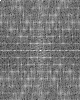
\includegraphics[width=2cm]{wrong/dft_mag}
\caption{amplitude}
 \end{figure}
        \end{minipage}
\begin{minipage}[t]{0.3\linewidth}
\begin{figure}
   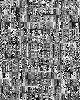
\includegraphics[width=2cm]{wrong/dft_phase}
\caption{phase}
 \end{figure}
        \end{minipage}
\begin{minipage}[t]{0.3\linewidth}
\begin{figure}
   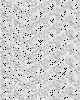
\includegraphics[width=2cm]{wrong/idft_shift}
\caption{idft}
 \end{figure}
        \end{minipage}
\end{frame}

% ----------------------------------------------------------------------------
\usebackgroundtemplate{
   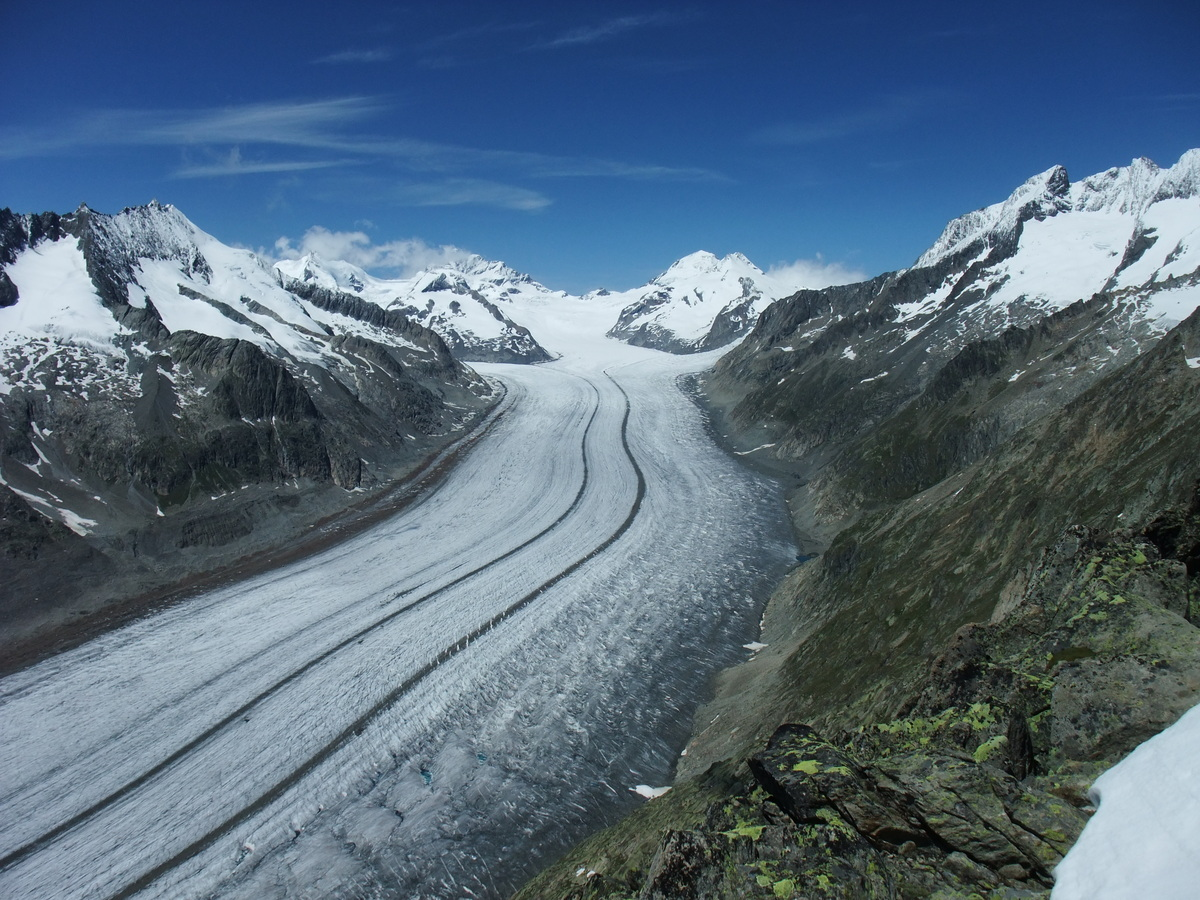
\includegraphics[width=\paperwidth,
                    height=\paperheight]{aletsch}
}
\begin{frame}
\ \\ \ \\
\centering \Large \textcolor{white}{Perhaps no questions...T.T}

\end{frame}
\usebackgroundtemplate{}
% ----------------------------------------------------------------------------


\end{document}
